Sistemas baseados em agentes podem ser modelados de forma similar a sistemas orientados a objeto, sendo que seus agentes tomam forma de objeto e passam a ser constituídos por atributos e métodos podendo se comunicar invocando métodos de outros agentes ou trocando mensagens, e podendo utilizar conceitos clássicos de orientação a objeto, como herança, encapsulamento e agregação de dados \cite{intelligent}. Em consequência disso, métodos relacionados ao desenvolvimento de aplicativos orientados a objeto formam a base de boa parte dos métodos de desenvolvimento de sistemas baseados em agentes. De forma similar a técnica para modelagem orientada a objeto proposta por \citeonline{OMT} que consiste de modelo básico, modelo estático e modelo dinâmico, \citeonline{agent-oriented} divide a análise orientada a agentes em três modelos, o modelo de agente, o modelo organizacional e o modelo cooperativo, descritos a seguir:

\begin{itemize}
  \item O modelo de agente contém descrições e estruturas internas dos agentes, descritas em termos de noções mentais como metas planos e crenças ou quaisquer estruturas que sejam apropriadas a arquitetura específica dos agentes sendo desenvolvidos. Esse modelo se assemelha ao modelo básico de métodos orientados a objeto;
  \item O modelo organizacional especifica os relacionamentos entre agentes e seus tipos. Estes são em parte relações de herança, e também relacionamentos entre agentes baseados em seus respectivos papéis em organizações. Essas organizações podem ser meios para estruturar sistemas complexos em subsistemas (assim como é feito em certas técnicas de orientação a objeto) ou podem ser usadas para modelar organizações reais. Esse modelo é semelhante ao modelo estático, mas como papéis podem mudar com o passar do tempo, ele não é um modelo genuinamente estático;
  \item O modelo cooperativo descreve a interação, ou mais especificamente, a cooperação entre os agentes. Este modelo contém apenas os \hyphenation{relacio-namentos} relacionamentos entre objetos. O processo que ocorre dentro dos objetos é representado pelo modelo de agente.
\end{itemize}


\subsection{Metodologias para Modelagem de Agentes}
A partir dos conceitos de modelagem de agentes apresentados, foram elaboradas diversas metodologias para a concep��o e o desenvolvimento destes agentes. Em fun��o da sua utilidade em rela��o ao desenvolvimento de agentes \emph{BDI}, sem deixar de ser �til para qualquer outro tipo de sistema multiagente, a metodologia utilizada no decorrer deste trabalho � a chamada \emph{Prometheus} \cite{prometheus}.

A metodologia \emph{Prometheus} consiste de tr�s fases, descritas por \citeonline{prometheus} da seguinte forma:
\begin{itemize}
  \item Especifica��o de Sistema: � focada em identificar as funcionalidades b�sicas do sistema como um todo, tais como suas entradas (percep��es), sa�das (a��es), e quaisquer fontes importantes de dados compartilhados;
  \item Modelagem Arquitetural: utiliza as sa�das da fase anterior para determinar quais agentes o sistema conter� e como eles ir�o interagir;
  \item Modelagem Detalhada: � onde s�o especificados os componentes internos de cada agente e como tal agente realizar� suas tarefas dentro do sistema.
\end{itemize}

Na figura 5 demonstra estas tr�s fases citadas acima de forma expl�cita, mostrando os artefatos gerados por cada fase, bem como os eventos que levam de uma fase a outra.

\begin{figure}[!htb]
	\centering
	\caption{Diagrama explicitando as fases da metodologia \emph{Prometheus}, obtido de \cite{prometheus}.}\label{fig:promehteus}
	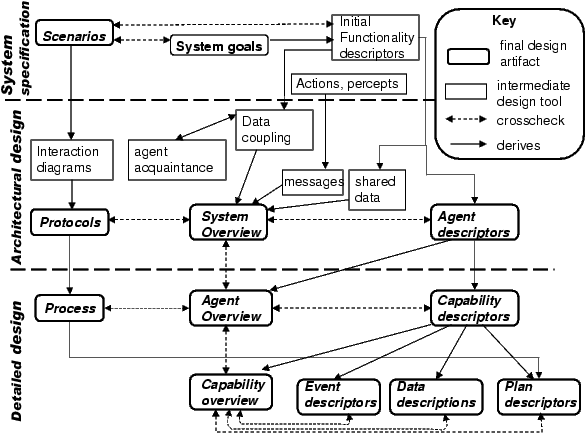
\includegraphics[width=1\textwidth]{figuras/prometheus.png}
\end{figure}

Vale notar que estas fases descritas acima e explicitadas na figura 5 constituem um processo iterativo de engenharia de software, e n�o um modelo de desenvolvimento do tipo cascata, sendo que estas fases n�o devem ser necessariamente executadas em alguma ordem em particular. \citeonline{prometheus} sugerem repetir o processo inteiro mais de uma vez, com um foco diferente a cada repeti��o, sendo que a primeira itera��o pode consistir inteiramente de atividades associadas a fase de especifica��o de sistema, itera��es subsequentes envolver�o uma mistura de atividades de fases diferentes, eventualmente com uma presen�a maior de atividades das fases seguintes.


\subsection{Ferramentas para Modelagem de Agentes}
Dentre as ferramentas para modelagem de agentes dispon�veis, a \emph{Prometheus Design Tool} \cite{pdt} chama aten��o por ter sido elaborada em conjunto com os autores da metodologia \emph{Prometheus}, justamente para complementar a metodologia.

A \emph{Prometheus Design Tool} � baseada em caracter�sticas espec�ficas de agentes como metas, planos, percep��es, a��es e protocolos e � estruturada em torno das tr�s fases da metodologia \emph{Prometheus} descritas anteriormente \cite{pdt}. Al�m do suporte ao desenvolvimento gr�fico de diagramas de \emph{design} para o sistema multiagente, \citeonline{pdt} citam diferentes atributos da ferramenta, sendo alguns dos mais not�veis destes:

\begin{itemize}
  \item Verifica��o de Consist�ncia: a ferramenta mant�m restri��es baseados em um meta-modelo, providenciando suporte � preven��o de erros simples como a gera��o de uma entidade indesejada causada por um erro de digita��o;
  \item Propaga��o: sempre que poss�vel, informa��es s�o propagadas de uma parte do modelo para outra. Por exemplo, se um conjunto de metas � associado a um papel, e esse papel � associado a um agente, ent�o as metas ser�o automaticamente associadas ao agente;
  \item Testes Automatizados: a ferramenta suporta a gera��o e execu��o automatizadas de testes de unidade para eventos, cren�as e planos, baseados no modelo.
\end{itemize}

